\section{Análise do Conjunto de Dados}
\label{sec:geral}

Antes de aplicar os algoritmos descritos anteriormente, é possível obter algumas informações do conjunto de dados. Existem 604.315 casos registrados, onde 94,91\% são casos leves e os restantes são considerados graves, destes, 25,15\% resultaram em óbito. Destes casos, embora o total seja de 43,5\% para o sexo masculino, eles consistem em 49,3\% dos casos graves. O sintoma mais comum foi a tosse, presente em 38\% de todos os casos e 72\% dos casos graves. Mapas de calor de correlação estão disponíveis nos apêndices \ref{apendice:correlacao}, \ref{apendice:correlacao-v0} e \ref{apendice:correlacao-v30}. As tabelas abaixo destrincham a distribuição da severidade dos casos e óbitos, de acordo com o Progresso de Vacinação e Idade.


  \begin{table}[H]
    \centering
    \begin{tabular}{|c|c|c|c|c|c|c|c|c|}
    \hline
    \textbf{Vacinação}          & \textbf{Total} & \textbf{\%} & \textbf{Leves} & \textbf{\%} & \textbf{Graves} & \textbf{\%} & \textbf{Óbitos} & \textbf{\%} \\ \hline
    \textbf{=0\%}               & 272144         & 45.64\%           & 251882         & 91.03\%           & 15689           & 5.67\%             & 4573            & 1.65\%             \\ \hline
    \textbf{\textgreater{}0\%}  & 332171         & 54.97\%           & 321697         & 95.93\%           & 7315            & 2.18\%             & 3159            & 0.94\%             \\ \hline
    \textbf{\textgreater{}15\%} & 260258         & 43.07\%           & 252035         & 95.93\%           & 5749            & 2.19\%             & 2474            & 0.94\%             \\ \hline
    \textbf{\textgreater{}30\%} & 188579         & 31.21\%           & 182667         & 95.95\%           & 4118            & 2.16\%             & 1794            & 0.94\%             \\ \hline
    \textbf{\textgreater{}45\%} & 112003         & 18.53\%           & 108533         & 95.97\%           & 2381            & 2.11\%             & 1089            & 0.96\%             \\ \hline
    \textbf{\textgreater{}60\%} & 36072          & 5.97\%            & 34891          & 95.76\%           & 816             & 2.24\%             & 365             & 1.00\%             \\ \hline
    \end{tabular}
    \caption{Quantidade de casos leves, graves e óbitos por progresso de vacinação}
    \label{tbl:tabela-vacina-severidade}
    \end{table}
    
\begin{table}[H]
  \centering
  \begin{tabular}{|c|c|c|c|c|c|c|}
  \hline
  \textbf{Idade} & \textbf{Leves} & \textbf{\%} & \textbf{Graves} & \textbf{\%} & \textbf{Óbitos} & \textbf{\%} \\ \hline
  \textbf{0-9}   & 21260          & 89.68\%           & 2365            & 9.98\%             & 41              & 0.17\%             \\ \hline
  \textbf{10-19} & 36142          & 98.63\%           & 465             & 1.27\%             & 19              & 0.05\%             \\ \hline
  \textbf{20-29} & 107641         & 98.27\%           & 1702            & 1.55\%             & 96              & 0.09\%             \\ \hline
  \textbf{30-39} & 130232         & 97.02\%           & 3457            & 2.58\%             & 272             & 0.20\%             \\ \hline
  \textbf{40-49} & 111150         & 95.68\%           & 3882            & 3.34\%             & 570             & 0.49\%             \\ \hline
  \textbf{50-59} & 83865          & 92.95\%           & 3979            & 4.41\%             & 1191            & 1.32\%             \\ \hline
  \textbf{60-69} & 51814          & 88.49\%           & 3145            & 5.37\%             & 1796            & 3.07\%             \\ \hline
  \textbf{70-79} & 22328          & 79.54\%           & 2224            & 7.92\%             & 1760            & 6.27\%             \\ \hline
  \textbf{80+}   & 9147           & 61.25\%           & 1758            & 11.77\%            & 2014            & 13.49\%            \\ \hline
  \end{tabular}
  \caption{Quantidade de casos leves, graves e óbitos por idade}
  \label{tbl:tabela-idade-severidade}
  \end{table}

As figuras \ref{fig:plot-sev} e \ref{fig:plot-obt} comparam a distribuição da porcentagem de casos graves e óbitos, respectivamente, pelas categorias de idade e progresso da vacinação.

\begin{figure}[ht!]
  \centering
  \fcolorbox{white}{white}{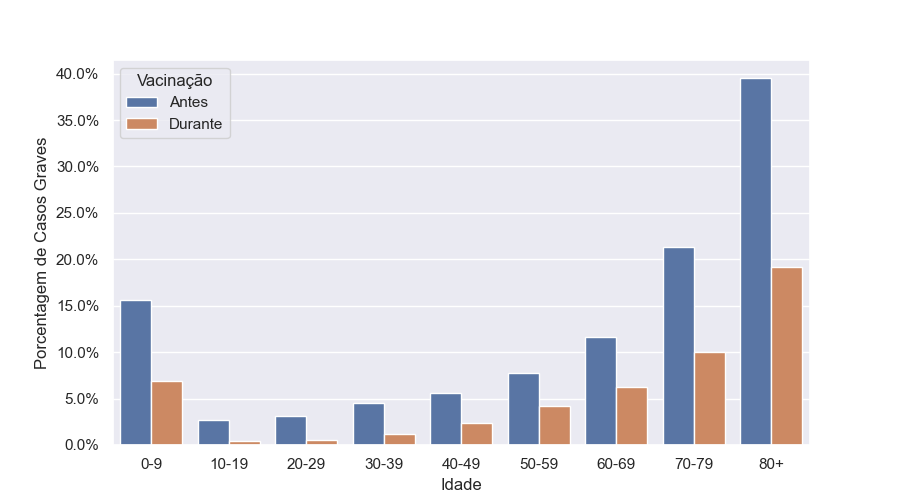
\includegraphics[width=0.65\textwidth]{chapters/resultados/images/plot_idade_severidade_vacina.png}}
  \caption{\textmd{Gráfico da porcentagem de casos graves para idades e vacinação}}
  \label{fig:plot-sev}
\end{figure}

\begin{figure}[ht!]
  \centering
  \fcolorbox{white}{white}{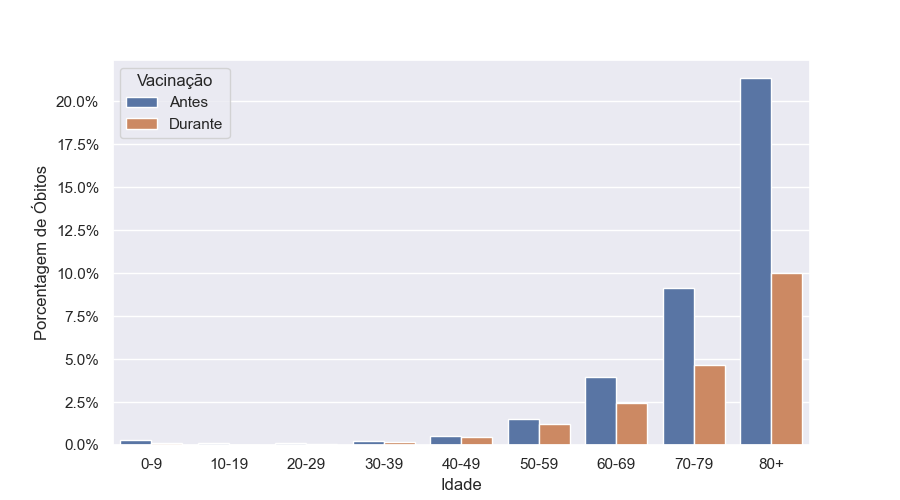
\includegraphics[width=0.65\textwidth]{chapters/resultados/images/plot_idade_obito_vacina.png}}
  \caption{\textmd{Gráfico da porcentagem de óbitos para idades e vacinação}}
  \label{fig:plot-obt}
\end{figure}

